\documentclass[12pt]{article}
\usepackage[a4paper, total={21cm, 29.7cm}, margin=3cm]{geometry}
\usepackage{times}    % times new roman font
\usepackage{amsmath}
\usepackage{listings} % cool ah code
\usepackage{color}    % more cool shit code
\usepackage{graphicx} % fancy ah figure
\usepackage{float}    % forcing figure to float
\usepackage{enumitem}
\usepackage{lipsum} % sampling
\usepackage{setspace}
\usepackage{mdframed}
\usepackage{indentfirst} 
\usepackage{hyperref} % actually used for email and links, but kinda broken. (not used)
\usepackage{tabularx} % just because, but now more often use longtable
\usepackage{longtable} % cool table with it speciality to be able cut along 2 page
\usepackage{multirow} % merge row
\usepackage{tocloft} % table of content
\usepackage{rotating} % rotating figure
\usepackage{caption} % need to explain?
\usepackage[none]{hyphenat} % no linebreak with -
\usepackage{showframe} % debugging
\usepackage{natbib} % bib cite stuff

% \usepackage{cite}
% \bibliographystyle{abbrvnat}
\setcitestyle{open={(},close={)}} %Citation-related commands


\usepackage{titlesec}

\titleformat{\section}{\filcenter\normalfont\large\bfseries}{}{1em}{} 

\DeclareCaptionLabelFormat{nospace}{#1#2}
\captionsetup[table]{name=Tabel }
\captionsetup[figure]{name=Gambar }
\renewcommand{\thefigure}{\thesection.\arabic{figure}}
\renewcommand{\thetable}{\thesection.\arabic{table}}

\usepackage{tocloft}
\setlength{\cftbeforeloftitleskip}{0em} % Adjust spacing if necessary
\setlength{\cftbeforelottitleskip}{0em}

\renewcommand{\refname}{DAFTAR PUSTAKA}
\renewcommand{\contentsname}{\center DAFTAR ISI}
\renewcommand{\listfigurename}{DAFTAR GAMBAR}
\renewcommand{\listtablename}{DAFTAR TABEL}

\usepackage{etoolbox}
\patchcmd{\listoffigures}{\section*}{\section*{\centering}}{}{}
\patchcmd{\listoftables}{\section*}{\section*{\centering}}{}{}

% for list
\setlist{  
  listparindent=\parindent,
  parsep=0pt,
}
\newcommand{\listsection}[1]{
    \item \textbf{#1}
    \addcontentsline{toc}{section}{#1}
}


\setlength\parindent{2.5em}
\setlength{\emergencystretch}{2.5em}

\renewcommand{\baselinestretch}{1.2}
\renewcommand*{\arraystretch}{1.2} 
\setlength{\extrarowheight}{.2ex}

\definecolor{dkgreen}{rgb}{0,0.6,0}
\definecolor{gray}{rgb}{0.5,0.5,0.5}
\definecolor{mauve}{rgb}{0.58,0,0.82}

\lstset{frame=tb,
    language=Python,
    aboveskip=3mm,
    belowskip=3mm,
    showstringspaces=true,
    columns=flexible,
    basicstyle={\small\ttfamily},
    numbers=none,
    numberstyle=\tiny\color{gray},
    keywordstyle=\color{blue},
    commentstyle=\color{dkgreen},
    stringstyle=\color{mauve},
    breaklines=true,
    breakatwhitespace=true,
    tabsize=4
}

\def\mynewrule#1{\hbox to #1in{\leaders\hbox to 0.00625in{\hfil.\hfil}\hfill}}
%%%%Defined the signature line with \hfill%%%   
\def\rnewrule#1{\hfill\mynewrule{#1}}
%%%%Defined block to include rule and information%%%
\def\rsignblock#1#2{
    \hfill
    \vtop{
        \hsize=#1in
        \noindent{Semarang, ...}\par
        \vspace*{2cm}
        \noindent{#2}\par
    }
    \par
    \hfill
    % \rnewrule{#1}\par     
    \vskip1cm
}

\begin{document}
\begin{titlepage}
    \begin{center}
        {
            % \setstretch{2}
            \textbf{ LAPORAN PRAKTEK KERJA LAPANGAN} \\
            \textbf{SISTEM MANAJEMEN PRODUK DAN TICKETING}\\
            \textbf{ BAGIAN MODUL TICKETING} \\
            \textbf{DI PT TEKNOLOGI APLIKASI SEJAHTERA} \\
        }

        \vfill
        
\includegraphics[width=4cm]{images/logo-undip.png} \\
        \vfill
        \textbf{ Disusun Oleh:} \\
        Givandra Haikal Adjie \\
        240601211130063 \\

        \vspace{1cm}
        \textbf{
        DEPARTEMEN NFORMATIKA \\
        FAKULTAS SAINS DAN MATEMATIKA \\
        UNIVERSITAS DIPONEGORO \\
        SEMARANG \\
        2023}

    \end{center}
\end{titlepage}



% HALAMAN PENGESAHAN
%  ██      ██     ██     ██           ██     ████     ████     ██     ████     ██
% ░██     ░██    ████   ░██          ████   ░██░██   ██░██    ████   ░██░██   ░██
% ░██     ░██   ██░░██  ░██         ██░░██  ░██░░██ ██ ░██   ██░░██  ░██░░██  ░██
% ░██████████  ██  ░░██ ░██        ██  ░░██ ░██ ░░███  ░██  ██  ░░██ ░██ ░░██ ░██
% ░██░░░░░░██ ██████████░██       ██████████░██  ░░█   ░██ ██████████░██  ░░██░██
% ░██     ░██░██░░░░░░██░██      ░██░░░░░░██░██   ░    ░██░██░░░░░░██░██   ░░████
% ░██     ░██░██     ░██░████████░██     ░██░██        ░██░██     ░██░██    ░░███
% ░░      ░░ ░░      ░░ ░░░░░░░░ ░░      ░░ ░░         ░░ ░░      ░░ ░░      ░░░
%  ███████  ████████ ████     ██   ████████  ████████  ████████     ██      ██      ██     ██     ████     ██
% ░██░░░░██░██░░░░░ ░██░██   ░██  ██░░░░░░██░██░░░░░  ██░░░░░░     ████    ░██     ░██    ████   ░██░██   ░██
% ░██   ░██░██      ░██░░██  ░██ ██      ░░ ░██      ░██          ██░░██   ░██     ░██   ██░░██  ░██░░██  ░██
% ░███████ ░███████ ░██ ░░██ ░██░██         ░███████ ░█████████  ██  ░░██  ░██████████  ██  ░░██ ░██ ░░██ ░██
% ░██░░░░  ░██░░░░  ░██  ░░██░██░██    █████░██░░░░  ░░░░░░░░██ ██████████ ░██░░░░░░██ ██████████░██  ░░██░██
% ░██      ░██      ░██   ░░████░░██  ░░░░██░██             ░██░██░░░░░░██ ░██     ░██░██░░░░░░██░██   ░░████
% ░██      ░████████░██    ░░███ ░░████████ ░████████ ████████ ░██     ░██ ░██     ░██░██     ░██░██    ░░███
% ░░       ░░░░░░░░ ░░      ░░░   ░░░░░░░░  ░░░░░░░░ ░░░░░░░░  ░░      ░░  ░░      ░░ ░░      ░░ ░░      ░░░

\newpage


%      ██     ██████    ████████ ██████████ ███████       ██     ██   ██
%     ████   ░█░░░░██  ██░░░░░░ ░░░░░██░░░ ░██░░░░██     ████   ░██  ██
%    ██░░██  ░█   ░██ ░██           ░██    ░██   ░██    ██░░██  ░██ ██
%   ██  ░░██ ░██████  ░█████████    ░██    ░███████    ██  ░░██ ░████
%  ██████████░█░░░░ ██░░░░░░░░██    ░██    ░██░░░██   ██████████░██░██
% ░██░░░░░░██░█    ░██       ░██    ░██    ░██  ░░██ ░██░░░░░░██░██░░██
% ░██     ░██░███████  ████████     ░██    ░██   ░░██░██     ░██░██ ░░██
% ░░      ░░ ░░░░░░░  ░░░░░░░░      ░░     ░░     ░░ ░░      ░░ ░░   ░░
\newpage

%      ██     ██████    ████████ ██████████ ███████       ██       ██████   ██████████
%     ████   ░█░░░░██  ██░░░░░░ ░░░░░██░░░ ░██░░░░██     ████     ██░░░░██ ░░░░░██░░░
%    ██░░██  ░█   ░██ ░██           ░██    ░██   ░██    ██░░██   ██    ░░      ░██
%   ██  ░░██ ░██████  ░█████████    ░██    ░███████    ██  ░░██ ░██            ░██
%  ██████████░█░░░░ ██░░░░░░░░██    ░██    ░██░░░██   ██████████░██            ░██
% ░██░░░░░░██░█    ░██       ░██    ░██    ░██  ░░██ ░██░░░░░░██░░██    ██     ░██
% ░██     ░██░███████  ████████     ░██    ░██   ░░██░██     ░██ ░░██████      ░██
% ░░      ░░ ░░░░░░░  ░░░░░░░░      ░░     ░░     ░░ ░░      ░░   ░░░░░░       ░░


\newpage

\begin{center}
    \textbf{\large KATA PENGANTAR} \\
\end{center}

Puji syukur penulis panjatkan kepada Tuhan Yang Maha Esa atas segala berkat rahmat dan hikmat-Nya penulis dapat menyelesaikan Laporan Praktek Kerja Lapangan “Sistem Manajemen Produk dan Ticketing bagian Modul Dashboard di PT Teknologi Aplikasi Sejahtera”. Penulis menyadari dalam menyelesaikan kegiatan PKL ini sangatlah sulit tanpa bantuan dan bimbingan dari berbagai  pihak. Bersama ini, penulis menyampaikan terima kasih kepada:

\begin{enumerate} %[label=\textbf{1.\arabic*}]
    \item Bapak Prof. Dr. Yos Johan Utama, S.H., M.Hum, selaku RektorUniversitas Diponegoro Semarang;

    \item Ibu Prof. Dr. Widowati, S.Si., M.Si., selaku dekan Fakultas Sains dan Matematika yang telah memberikan izin untuk melakukan Praktek Kerja Lapangan di PT Teknologi Aplikasi Sejahtera;

    \item Bapak Dr. Aris Puji Widodo, S.Si, M.T. selaku Ketua Departemen Informatika yang telah membantu dalam proses perizinan PKL di PT Teknologi Aplikasi Sejahtera;

    \item Ibu Beta Noranita, S.Si., M.Kom. selaku Dosen Pembimbing PKL yang telah membimbing penulis hingga terselesaikannya PKL ini;

    \item Bapak Sandy Kurniawan, S.Kom., M.Kom. selaku Koordinator PKL Departemen Informatika yang telah memberikan bimbingan serta arahan mengenai pelaksanaan PKL;

    \item PT Teknologi Aplikasi Sejahtera;

    \item Serta semua pihak yang telah terlibat membantu kelancaran dan pelaksanaan dalam kegiatan ini.

\end{enumerate}

Penulis menyadari bahwa masih banyak kekurangan dalam laporan PKL ini. Maka dari itu, saran dan kritik yang membangun sangat penulis harapkan. Semoga laporan ini dapat bermanfaat bagi semua pihak.

\vspace*{2cm}

\rsignblock{2}{Givandra Haikal Adjie}

\newpage

\tableofcontents

\newpage

\listoffigures

\newpage

\listoftables

\newpage


\section{BAB I\\PENDAHULUAN}
% \addcontentsline{toc}{section}{BAB I PENDAHULUAN}
% \begin{center}
% {
%     \setstretch{2}
%     \textbf{\large BAB I} \\
%     \textbf{\large PENDAHULUAN} \\
% }
% \end{center}

\begin{enumerate}[label=\textbf{1.\arabic*.}]
    \listsection{Latar Belakang}
    \addcontentsline{toc}{section}{Latar Belakang}
    
    Kemajuan teknologi dan digitalisasi yang cepat telah memberikan banyak kemudahan dalam menjalankan pekerjaan, termasuk bagi perusahaan dan bisnis yang menggunakan teknologi dalam operasional mereka. Untuk tetap bersaing di pasar yang kompetitif, perusahaan harus terus beradaptasi dengan teknologi, termasuk dengan membangun berbagai sistem informasi untuk menjaga keunggulan mereka. PT Teknologi Aplikasi Sejahtera, sebuah perusahaan pengembang perangkat lunak, juga mengalami peningkatan dalam intensitas manajemen produk dan layanan pelanggan seiring dengan pertumbuhan perangkat lunak yang mereka hasilkan setiap tahunnya. 
    
    Namun, meskipun telah menghasilkan beragam aplikasi untuk kliennya, manajemen tiket dari klien masih dilakukan secara manual melalui WhatsApp dengan perantara salah satu karyawan disana yang mengurus bagian ini sebagai tugas tambahan. Hal ini menimbulkan tantangan efisiensi dalam mengakses informasi serta kesalahan manusia. 
    
    Oleh karena itu, diperlukan pembuatan sebuah sistem informasi berbasis web yang bertujuan untuk meningkatkan efisiensi dalam manajemen bug dan pelaporan, serta penyimpanan dokumentasi produk. Berdasarkan analisis awal, terdapat beberapa bagian yang dapat dikerjakan secara terpisah, salah satunya adalah modul ticketing yang akan difokuskan pada manajemen ticket. Modul ini mencakup pengelolaan tiket dari pembuatan, administrasi internal, hingga penutupan, serta berfungsi sebagai perantara antara pihak eksternal dan internal. Sistem informasi yang kami rencanakan akan menggunakan PHP dengan framework Laravel sebagai backend, PostgreSQL sebagai manajemen basis data, dan React.js sebagai frontend.

    \listsection{Rumusan Masalah}
    
    Berdasarkan latar belakang dan permasalahan yang telah dibahas, maka rumusan masalah dari proyek PKL ini adalah bagaimana merancang dan membuat Sistem Manajemen Produk dan Ticketing modul Ticketing di PT Teknologi Aplikasi Sejahtera.

    \listsection{Tujuan}
    
    Tujuan dilaksanakannya praktek kerja lapangan ini adalah untuk menghasilkan Sistem Manajemen Produk dan Ticketing PT Teknologi Aplikasi Sejahtera yang dapat membantu permasalahan pengelolaan ticket yang masih dilakukan secara manual. 

    \hspace*{1pt} % cringe space

    \listsection{Manfaat}

    Sedangkan untuk manfaat dilaksanakannya praktek kerja lapangan ini adalah agar PT Teknologi Aplikasi Sejahtera dapat menggunakan Sistem Manajemen Produk dan Ticketing ini dalam meningkatkan efisiensi dari mengelola ticket lebih baik serta menyediakan tempat untuk mengarsipkan ticket ticket yang sudah selesai secara terpusat.
    
    \listsection{Ruang Lingkup}
    
    Ruang lingkup dalam praktek kerja lapangan ini adalah Sistem Manajemen Produk dan Ticketing yang berfokus pada modul ticketing.
    
    \listsection{Sistematika Penulisan}

    Berdasarkan latar belakang dan permasalahan yang telah dibahas, maka berikut adalah rumusah masalah dari projek yang dibuat:

    \begin{enumerate}[listparindent=0pt, label=, ]
        \item BAB I PENDAHULUAN
    
        Bab ini berisikan mengenai informasi perusahaan tempat kegiatan Praktek Kerja Lapangan dilaksanakan, yaitu PT. Teknologi Aplikasi Sejahtera disertai dengan profil instansi, visi, misi, dan struktur organisasi. 
        
        \item BAB II LANDASAN TEORI
        
        Bab ini membahas mengenai landasan teori yang digunakan dalam pembangunan Laporan Praktek Kerja Lapangan pada Sistem Manajemen Produk dan Ticketing Pada PT. Teknologi Aplikasi Sejahtera. 
        
        \item BAB III ANALISIS KEBUTUHAN DAN PERANCANGAN
        
        Bab ini menjelaskan tentang pembahasan yang meliputi deskripsi umum perangkat lunak, analisis, dan desain rancangan Laporan Praktek Kerja Lapangan pada Sistem Manajemen Produk dan Ticketing Pada PT. Teknologi Aplikasi Sejahtera.
        
        \item BAB IV IMPLEMENTASI DAN PENGUJIAN
        
        Bab ini menjelaskan mengenai implementasi berdasarkan rancangan sistem dan pengujian dari sistem yang telah dibentuk, yaitu Laporan Praktek Kerja Lapangan pada Sistem Manajemen Produk dan Ticketing Pada PT. Teknologi Aplikasi Sejahtera.
        
        \item BAB V PENUTUP
        
        Bab ini membahas kesimpulan dari Praktek Kerja Lapangan yang sudah dilakukan dan saran penulis untuk pengembangan lebih lanjut mengenai sistem yang telah dibuat.
    \end{enumerate}
\end{enumerate}

\newpage

\section{BAB II\\TINJAUAN PERUSAHAAN}
% \begin{center}
% {
%     \setstretch{2}
%     \textbf{\large BAB II} \\
%     \textbf{\large TINJAUAN PERUSAHAAN} \\
% }
% \end{center}

Bagian ini akan membahas terkait dengan informasi seputar PT. Teknologi Aplikasi Sejahtera yang berupa profil instansi, visi dan misi, serta struktur organisasinya. 

\begin{enumerate}[label=\textbf{2.\arabic*.}]
    \listsection{Profil Instansi}

    PT Teknologi Aplikasi Sejahtera (TAS) merupakan perusahaan pengembang teknologi yang berkantor di Semarang, PT Teknologi Aplikasi Sejahtera berkomitmen untuk menjadi perusahaan teknologi informasi terintegrasi dengan support system yang unggul, inovatif dan terpercaya. PT Teknologi Aplikasi Sejahtera menyediakan layanan pembuatan web apps, mobile apps, hingga IoT (Internet Of Things). Informasi detail terkait dengan PT Teknologi Aplikasi Sejahtera dapat dilihat pada tabel 2.1 dibawah ini.

    \begin{table}[h!]
        \centering
        \begin{tabularx}{\linewidth}{ |l|X| }
            \hline
            Nama Instansi & PT Teknologi Aplikasi Sejahtera \\ %\addlinespace
            \hline
            Alamat Kantor & Jl. Plamongan Indah Blok E2 No. 17, Batursari, Kec. Mranggen, Kabupaten Demak 59567 \\ %\addlinespace
            \hline
            Telepon       & 0895-3271-75587 \\ %\addlinespace
            \hline
            Email         & teknosejahtera@gmail.com \\ %\addlinespace
            \hline
            Website       & https://teknosejahtera.co.id/ \\ %\addlinespace
            \hline
        \end{tabularx}
        \caption{Informasi PT Teknologi Aplikasi Sejahtera}
        \label{table:info}
    \end{table}

    \listsection{Visi}

    PT. Teknologi Aplikasi Sejahtera memiliki 4 Visi, yaitu:

        \begin{enumerate}[label=\arabic*.]
        \item \textit{Smart Innovation}
        \item \textit{Excellence Integration}
        \item \textit{Trust Integrity}
        \item \textit{Express Delivery Orientation}
    \end{enumerate}

    \listsection{Misi}

    PT Teknologi Sejahtera memiliki visi untuk menjadi perusahaan teknologi informasi terintegrasi yang terkemuka dengan support system yang unggul, inovatif dan terpercaya sehingga memberikan manfaat sebesar-besarnya bagi bangsa indonesia maupun pengguna secara luas dengan menjawab serta mempersiapkan kebutuhan

    \hspace*{1pt}

    \listsection{Struktur Organisasi}

    Pada gambar 2.1 di bawah ini merupakan struktur organisasi PT Teknologi Aplikasi Sejahtera. Dipimpin oleh Bapak Mardi Siswo Utomo selaku Direktur, dengan beberapa divisi di bawahnya, antara lain sekretaris, pengembangan bisnis, rumah tangga, keuangan, serta produksi dan teknis. Selama pelaksanaan praktek kerja lapangan, saya ditempatkan di divisi produksi dan teknis, di bawah bimbingan supervisor lapangan, Bapak Zidan Rafindra U. Fokus utama divisi ini adalah pada pengembangan sistem informasi.

    
\end{enumerate}

\newpage

\section{BAB III\\LANDASAN TEORI}
% \begin{center}
% {
%     \setstretch{2}
%     \textbf{\large BAB III} \\
%     \textbf{\large LANDASAN TEORI} \\
% }
% \end{center}



\begin{enumerate}[label=\textbf{3.\arabic*}]
    \listsection{Sistem Informasi}
    
    Sistem informasi (SI) merupakan penunjang penting dari proses bisnis sebuah organisasi yang memfasilitasi komunikasi dan koordinasi di antara berbagai area fungsional, dan memungkinkan pertukaran data serta akses data dengan mudah di seluruh proses bisnis (Rainer et al., 2005). SI memainkan peran penting dalam tiga bidang:

    
\end{enumerate}


\newpage
\section{BAB IV\\ANALISIS DAN PERANCANGAN}

% \begin{center}
% {
%     \setstretch{2}
%     \textbf{\large BAB IV} \\
%     \textbf{\large ANALISIS DAN PERANCANGAN} \\
% }
% \end{center}

\begin{enumerate}[label=\textbf{4.\arabic*.}]
    \listsection{Analisis Kebutuhan}

    Analisis kebutuhan digunakan untuk mengidentifikasi kebutuhan sistem yang akan dibangun. Pada bagian ini, terdapat penjelasan mengenai deskripsi umum sistem, kebutuhan fungsional, kebutuhan non-fungsional, use case diagram, activity diagram, dan sequence diagram

    \begin{enumerate}[label=\textbf{4.1.\arabic*.}, wide, labelwidth=!, labelindent=0pt]
        \listsection{Deskripsi Sistem}

        Sistem Informasi Manajemen Produk dan Ticketing bagian modul ticket di PT. Teknologi Aplikasi Sejahtera merupakan modul pengelolaan data bisnis dan transaksi yang berhubungan dengan manajemen ticketing yang ada di PT TAS. Dalam transaksi ticket ini ada beberapa role yang saling berinteraksi yakni internal user sebagai product manager, internal user sebagai developer, dan external user sebagai PIC pembuatan ticket. Ticket memiliki beberapa status yakni pending verification, in progress, done, closed dan rejected. Alur transaksi yang terjadi untuk setiap tahap ticket dapat dilihat sebagai berikut:

        \begin{enumerate}[label=\arabic*.]
            \item Pending verification
            
            Status ini merupakan status ketika ticket dibuat oleh external user dan menunggu verifikasi dari product manager apakah ticket ini valid atau tidak. Jika ticket ini valid, ticket akan dialokasikan developer yang akan mengerjakannya dan ticket akan berubah statusnya menjadi in progress. Jika ticket tidak valid, status ticket akan berubah menjadi rejected.
            
            \item In progress
            
            Ticket saat status ini sedang dikerjakan para developer, tiap developer yang mengerjakan ticket ini juga memiliki status pengerjaan yang dapat dilihat oleh user lain. Ketika semua developer sudah ok, product manager dapat mengecek apakah pengerjaan ticket sudah sesuai atau belum. Jika sesuai, ticket akan masuk ke tahap done untuk divalidasi pembuat ticket. Jika tidak sesuai, status pengerjaan developer akan direset dan status ticket tidak berubah.
            
            \item Done
            
            Ticket pada status ini akan dicek oleh external user apakah ticket yang sudah diajukan sudah benar benar sesuai. Jika terdapat ketidaksesuaian, external user dapat bisa mengajukan revisi dan ticket akan kembali menjadi in progress. Jika sesuai ticket akan menjadi closed.
            
            \item Closed
            
            Ticket dengan status ini berarti sudah selesai dan akan masuk ke dalam arsip.
            
            \item Rejected
            
            Ticket dengan status ini tidak sampai ke tahap pengerjaan dan masuk ke dalam arsip.
        \end{enumerate}


        \listsection{Kebutuhan Fungsional}

        Terdapat beberapa kebutuhan fungsional dari sistem dan pengguna untuk Sistem Informasi Manajemen Produk dan Ticketing bagian modul ticketing di PT. Teknologi Aplikasi Sejahtera. Daftar kebutuhan fungsional dapat dilihat pada tabel 4.1.

        \begin{longtable}{|l|p{0.7\textwidth}|}
            \hline
            \textbf{SRS ID} & \textbf{Deskripsi} \\
            \hline
            \endfirsthead
          
            \hline
            \textbf{SRS ID} & \textbf{Deskripsi} \\
            \hline
            \endhead
          
            SRS-TKT-PM-01 & Internal user (PM) dapat melihat list tiket yang dibuat oleh pihak eksternal berdasarkan product yang menjadi tanggung jawabnya \\
            \hline
            SRS-TKT-PM-02 & Internal user (PM) dapat memfilter list tiket berdasarkan status tiket \\
            \hline
            SRS-TKT-PM-03 & Internal user (PM) dapat melihat detail tiket yang sudah ada \\
            \hline
            SRS-TKT-PM-04 & Internal user (PM) dapat mem-verify tiket yang dibuat oleh pihak eksternal dan mengalokasikan developer yang bertanggung jawab \\
            \hline
            SRS-TKT-PM-05 & Internal user (PM) dapat menolak tiket yang dibuat oleh pihak eksternal dan memberikan alasan menolak \\
            \hline
            SRS-TKT-PM-06 & Internal user (PM) dapat mengusulkan revisi tiket yang sudah dikerjakan oleh developer dan memberikan alasan revisi \\
            \hline
            SRS-TKT-PM-07 & Internal user (PM) dapat berkomunikasi dengan pihak eksternal (pembuat tiket) melalui whatsapp \\
            \hline
            SRS-TKT-PM-08 & Internal user (PM) dapat mengubah status tiket menjadi done \\
            \hline
            SRS-TKT-DEV-01 & Internal user (DEV) dapat melihat list data tiket yang diassign oleh PM berdasarkan produk yang menjadi tanggung jawabnya \\
            \hline
            SRS-TKT-DEV-02 & Internal user (DEV) dapat memfilter list tiket berdasarkan status tiket \\
            \hline
            SRS-TKT-DEV-03 & Internal user (DEV) dapat melihat detail tiket yang sudah ada \\
            \hline
            SRS-TKT-DEV-04 & Internal user (DEV) dapat mengganti status pengerjaan tiket menjadi done dari tiket yang diassign oleh PM \\
            \hline
            SRS-TKT-PIC-01 & External user dapat melihat list tiket yang dibuat oleh dirinya berdasarkan product yang menjadi tanggung jawabnya \\
            \hline
            SRS-TKT-PIC-02 & External user dapat memfilter list tiket berdasarkan status tiket \\
            \hline
            SRS-TKT-PIC-03 & External user dapat membuat tiket baru berdasarkan produk yang menjadi tanggung jawabnya \\
            \hline
            SRS-TKT-PIC-04 & External user dapat melihat detail tiket yang telah dibuat \\
            \hline
            SRS-TKT-PIC-05 & External user dapat mengubah status tiket yang sudah selesai menjadi closed \\
            \hline
            SRS-TKT-PIC-06 & External user dapat mengubah status tiket yang sudah selesai kembali menjadi in progress jika masih ada yang belum terpenuhi \\
            \hline
            SRS-TKT-PIC-07 & External user dapat berkomunikasi dengan pihak internal (PM) melalui WA \\
            \hline
            \caption{Deskripsi SRS}
            \label{table:srs}
        \end{longtable}

        \listsection{Kebutuhan Non-Fungsional}

        Setelah mendapatkan kebutuhan fungsional, selanjutnya ada kebutuhan non-fungsional yang berfungsi sebagai fungsi pendukung dari fungsi utama atau kebutuhan fungsional sistem, berikut kebutuhan non-fungsional sistem yang dibuat dalam tabel 4.2.

        \begin{longtable}{|c|p{0.85\textwidth}|}
            \hline
            \textbf{No} & \textbf{Deskripsi} \\
            \hline
            \endfirsthead
          
            \hline
            \textbf{No} & \textbf{Deskripsi} \\
            \hline
            \endhead
          
            1 & Sistem harus kompatibel dan dapat dijalankan secara optimal di berbagai web browser seperti Google Chrome, Mozilla Firefox, Microsoft Edge, dan Safari \\
            \hline
            2 & Sistem harus memiliki response time yang tidak lebih dari 3 detik \\
            \hline
            3 & Sistem menggunakan standar enkripsi HTTPS \\
            \hline
            \caption{Deskripsi Sistem}
            \label{table:deskripsi-sistem}
        \end{longtable}

        \listsection{Daftar Use Case}

        Sistem Informasi Manajemen Produk dan Ticketing bagian ticketing di PT. Teknologi Aplikasi Sejahtera melibatkan beberapa use case. Deskripsi use case dijelaskan pada Tabel 4.3


        \begin{longtable}{|l|p{0.6\textwidth}|}
            \hline
            \textbf{Aktor} & \textbf{Deskripsi} \\
            \hline
            \endfirsthead
          
            \hline
            \textbf{Aktor} & \textbf{Deskripsi} \\
            \hline
            \endhead
          
            \multirow{8}{*}{Internal User (Product Manager)} 
            & Dapat melihat list tiket yang dibuat oleh pihak eksternal berdasarkan product yang menjadi tanggung jawabnya \\\cline{2-2}
            & Dapat memfilter list tiket berdasarkan status tiket \\\cline{2-2} 
            & Dapat melihat detail tiket yang sudah ada \\\cline{2-2}
            & Dapat mem-verify tiket yang dibuat oleh pihak eksternal dan 
            mengalokasikan developer yang bertanggung jawab \\\cline{2-2}
            & Dapat menolak tiket yang dibuat oleh pihak eksternal dan memberikan alasan menolak \\\cline{2-2}
            & Dapat mengusulkan revisi tiket yang sudah dikerjakan oleh developer dan memberikan alasan revisi \\\cline{2-2}
            & Dapat berkomunikasi dengan pihak eksternal (pembuat tiket) melalui whatsapp \\\cline{2-2}
            & Dapat mengubah status tiket menjadi done \\\cline{2-2}
            \hline
            \multirow{4}{*}{Internal User (Developer)} & Dapat melihat list data tiket yang diassign oleh PM berdasarkan produk yang menjadi tanggung jawabnya \\\cline{2-2}
            & Dapat memfilter list tiket berdasarkan status tiket \\\cline{2-2}
            & Dapat melihat detail tiket yang sudah ada \\\cline{2-2}
            & Dapat mengganti status pengerjaan tiket menjadi done dari tiket yang diassign oleh PM \\\cline{2-2}
            \hline
            \multirow{7}{*}{External User (PIC)} & Dapat melihat list tiket yang dibuat oleh dirinya berdasarkan product yang menjadi tanggung jawabnya \\\cline{2-2}
            & Dapat memfilter list tiket berdasarkan status tiket \\\cline{2-2}
            & Dapat membuat tiket baru berdasarkan produk yang menjadi tanggung jawabnya \\\cline{2-2}
            & Dapat melihat detail tiket yang telah dibuat \\\cline{2-2}
            & Dapat mengubah status tiket yang sudah selesai menjadi closed \\\cline{2-2}
            & Dapat berkomunikasi dengan pihak internal (PM) melalui WA \\\cline{2-2}
            \hline
            \caption{Deskripsi Aktor}
            \label{table:aktor}
        \end{longtable}
        
        \listsection{Use Case Diagram}

        Use case diagram adalah ilustrasi dari hubungan antara use case dengan aktor Admin yang ditunjukkan pada gambar \ref*{fig:example-figure}

        \begin{figure}[H]
            \centering 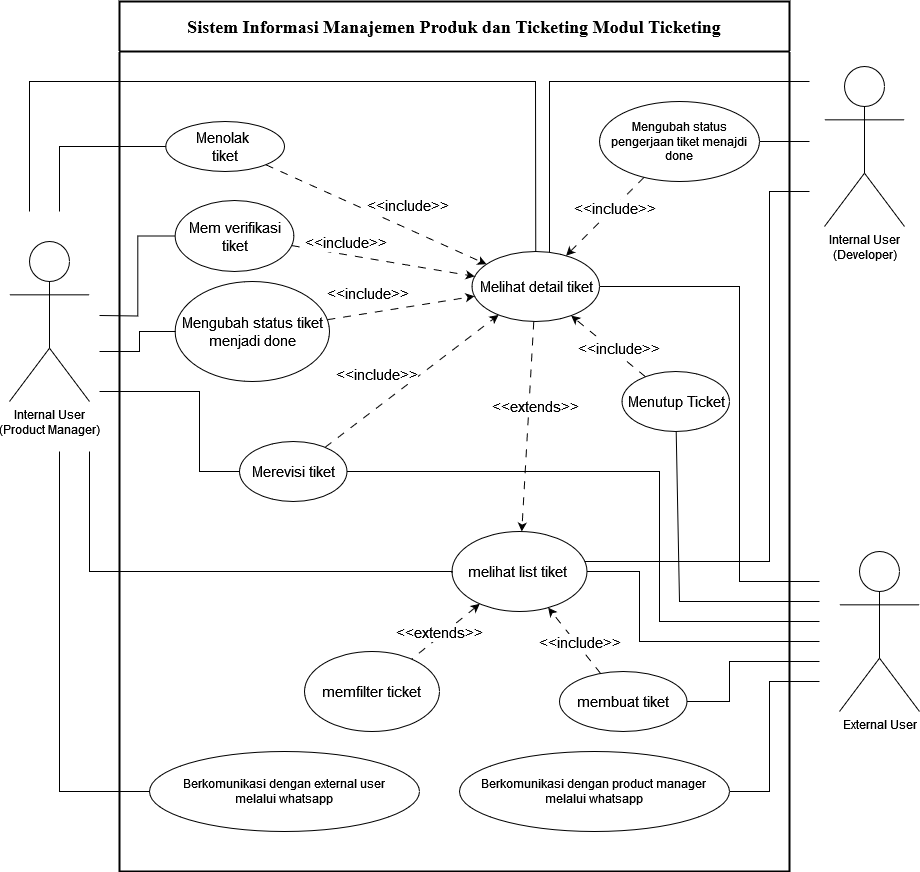
\includegraphics[width=\textwidth]{images/use-case.png}
            \caption{Descriptive Caption}
            \label{fig:example-figure}
        \end{figure}
    

        \listsection{Activity Diagram}

        \listsection{Sequence Diagram}

        Berdasarkan activity diagram yang telah dibuat, berikut adalah sequence diagram untuk Sistem Informasi Manajemen Produk dan Ticketing bagian ticketing di PT. Teknologi Aplikasi Sejahtera

        \begin{enumerate}[label=\textbf{4.1.7.\arabic*.}, wide, labelwidth=!, labelindent=0pt]
            \listsection{Sequence Diagram Internal User (Product Manager)}
            
            \begin{enumerate}[label=\arabic*., wide]
                \item Sequence Diagram Melihat List Ticket
                
                \begin{sidewaysfigure}
                    \centering 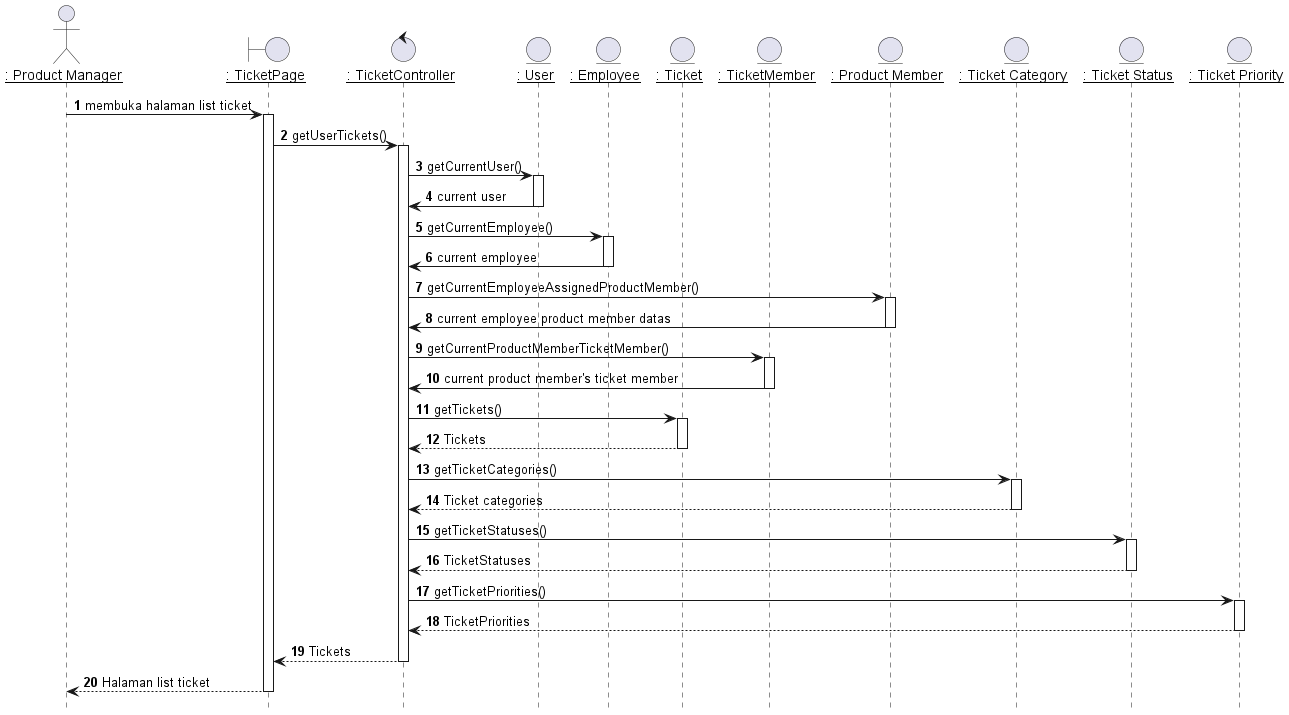
\includegraphics[width=\textwidth]{out/plantuml/sequence/ipm/ipm1/Melihat List Ticket.png}
                    \caption{Sequence Diagram Melihat List Ticket (External User)}
                    \label{fig:SQ-PM-01}
                \end{sidewaysfigure}

                \begin{sidewaysfigure}
                    \centering 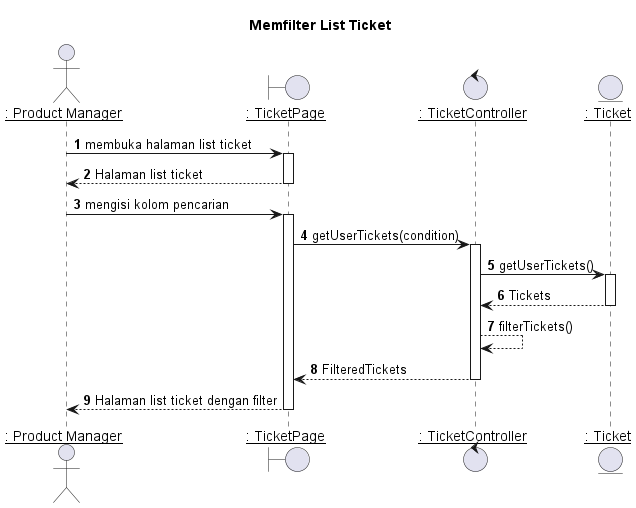
\includegraphics[width=\textwidth]{out/plantuml/sequence/ipm/ipm2/Memfilter List Ticket.png}
                    \caption{Sequence Diagram Memfilter List Ticket (External User)}
                    \label{fig:SQ-PM-02}
                \end{sidewaysfigure}

                \begin{sidewaysfigure}
                    \centering 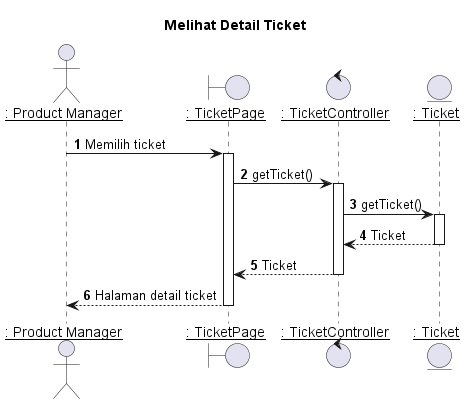
\includegraphics[width=\textwidth]{out/plantuml/sequence/ipm/ipm3/Melihat Detail Ticket.png}
                    \caption{Sequence Diagram Membuat Ticket (External User)}
                    \label{fig:SQ-PM-03}
                \end{sidewaysfigure}

                \begin{sidewaysfigure}
                    \centering 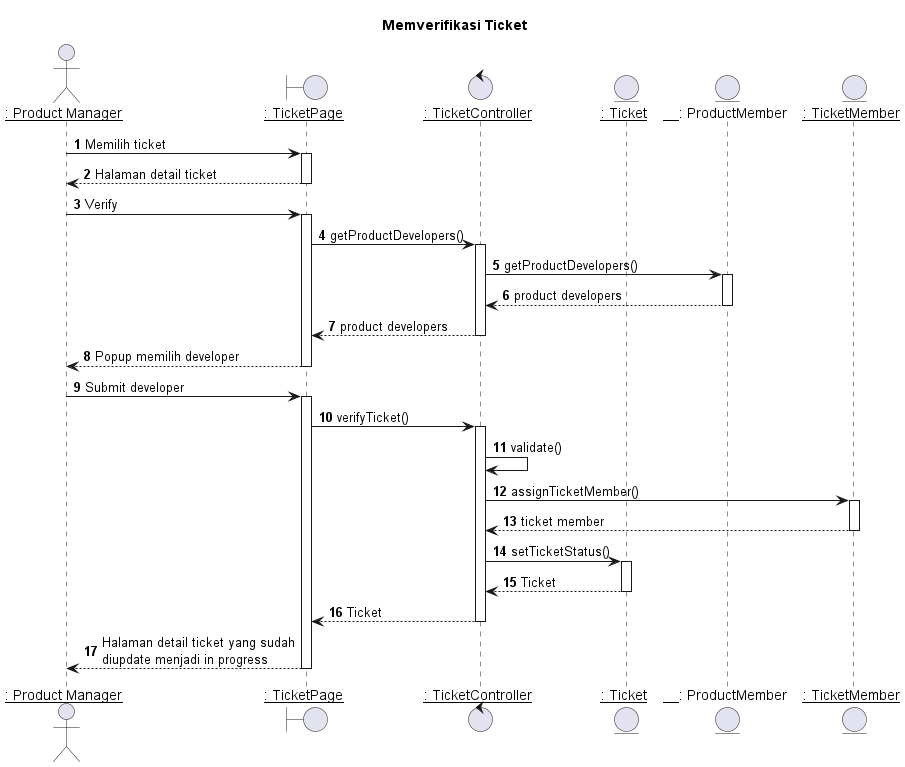
\includegraphics[width=\textwidth]{out/plantuml/sequence/ipm/ipm4/Memverifikasi Ticket.png}
                    \caption{Sequence Diagram Melihat Detail Ticket (External User)}
                    \label{fig:SQ-PM-04}
                \end{sidewaysfigure}

                \begin{sidewaysfigure}
                    \centering 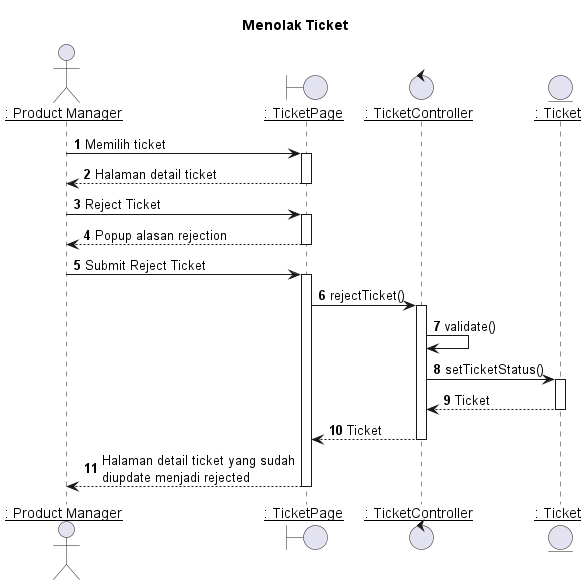
\includegraphics[width=\textwidth]{out/plantuml/sequence/ipm/ipm5/Menolak Ticket.png}
                    \caption{Sequence Diagram Menutup Ticket (External User)}
                    \label{fig:SQ-PM-05}
                \end{sidewaysfigure}

                \begin{sidewaysfigure}
                    \centering 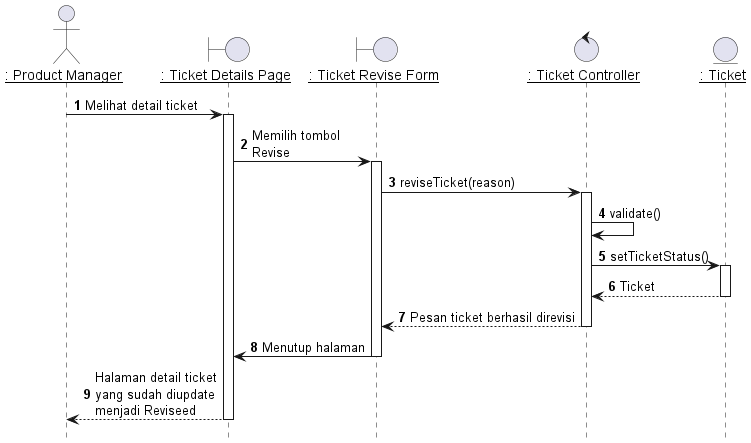
\includegraphics[width=\textwidth]{out/plantuml/sequence/ipm/ipm6/Merevisi Ticket.png}
                    \caption{Sequence Diagram Merevisi Ticket (External User)}
                    \label{fig:SQ-PM-06}
                \end{sidewaysfigure}

                \begin{sidewaysfigure}
                    \centering 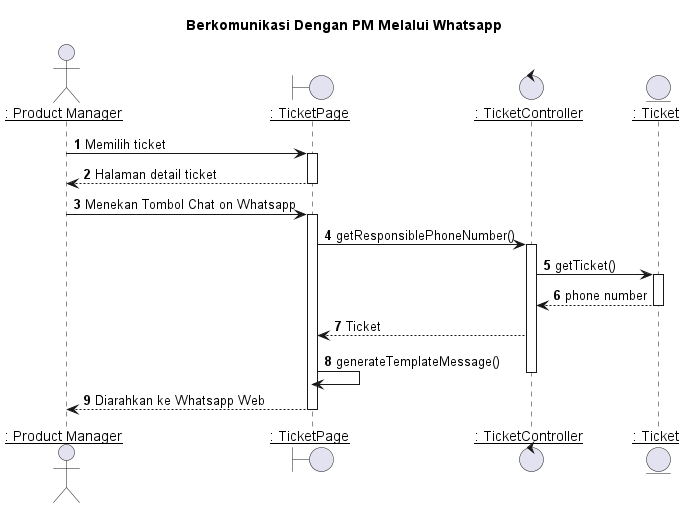
\includegraphics[width=\textwidth]{out/plantuml/sequence/ipm/ipm7/Berkomunikasi Dengan PM Melalui Whatsapp.png}
                    \caption{Sequence Diagram Berkomunikasi Dengan PM Melalui Whatsapp (External User)}
                    \label{fig:SQ-PM-07}
                \end{sidewaysfigure}

                \begin{sidewaysfigure}
                    \centering 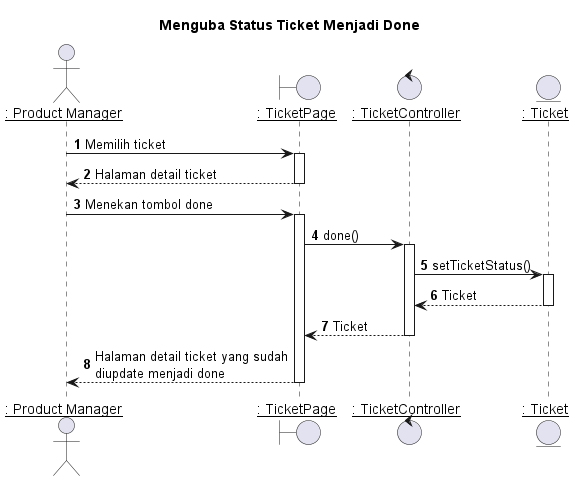
\includegraphics[width=\textwidth]{out/plantuml/sequence/ipm/ipm8/Menguba Status Ticket Menjadi Done.png}
                    \caption{Sequence Diagram Berkomunikasi Dengan PM Melalui Whatsapp (External User)}
                    \label{fig:SQ-PM-08}
                \end{sidewaysfigure}
            \end{enumerate}
            
            \listsection{Sequence Diagram Internal User (Developer)}
            
            \begin{enumerate}[label=\arabic*., wide]
                \item Sequence Diagram Melihat List Ticket
                
                \begin{sidewaysfigure}
                    \centering 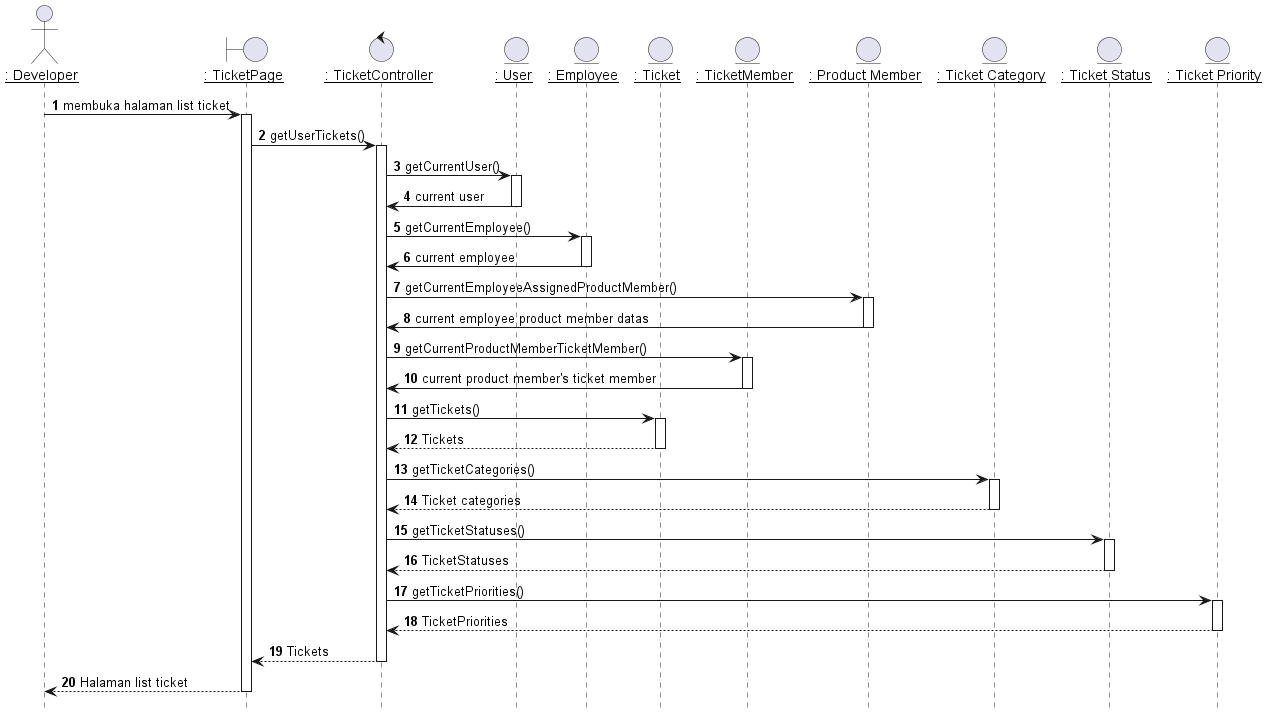
\includegraphics[width=\textwidth]{out/plantuml/sequence/idev/idev1/Melihat List Ticket.png}
                    \caption{Sequence Diagram Melihat List Ticket (DEV)}
                    \label{fig:SQ-DEV-01}
                \end{sidewaysfigure}

                \begin{sidewaysfigure}
                    \centering 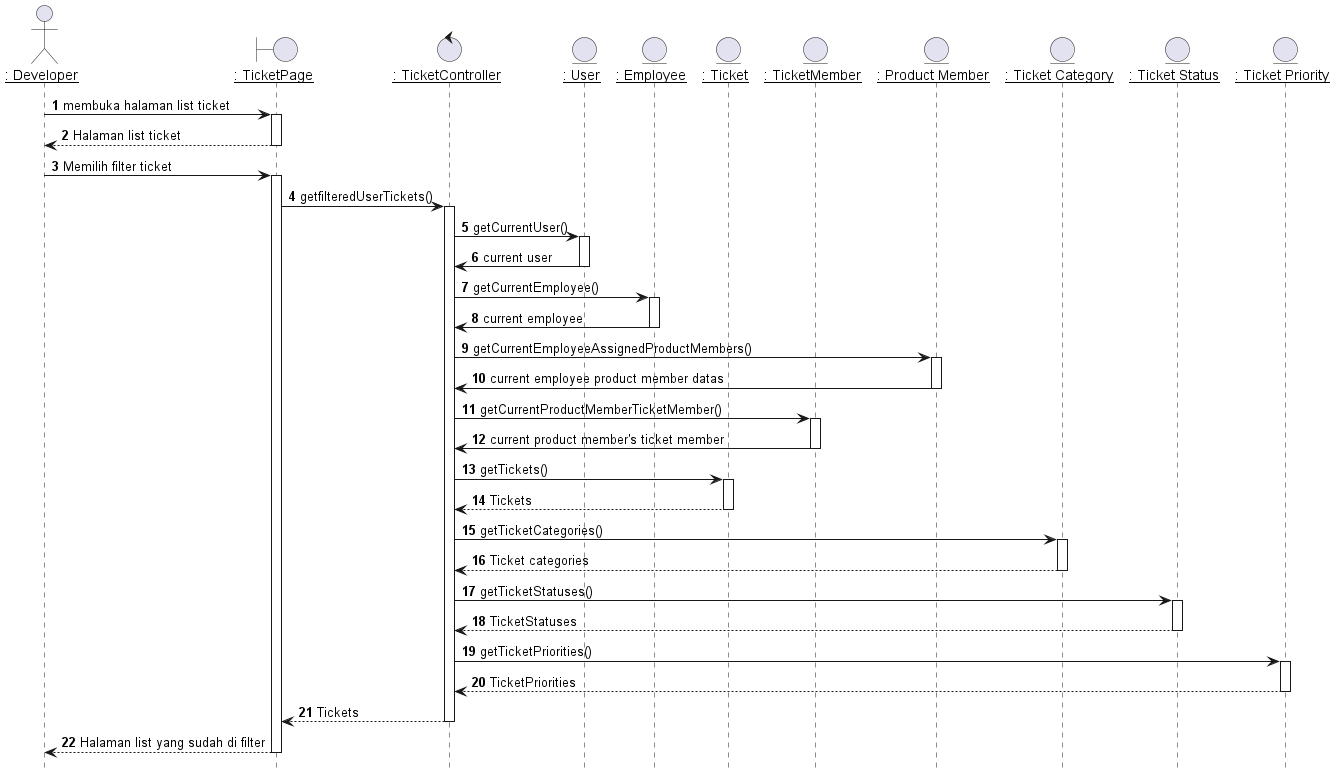
\includegraphics[width=\textwidth]{out/plantuml/sequence/idev/idev2/Memfilter List Ticket.png}
                    \caption{Sequence Diagram Memfilter List Ticket (DEV)}
                    \label{fig:SQ-DEV-02}
                \end{sidewaysfigure}

                \begin{sidewaysfigure}
                    \centering 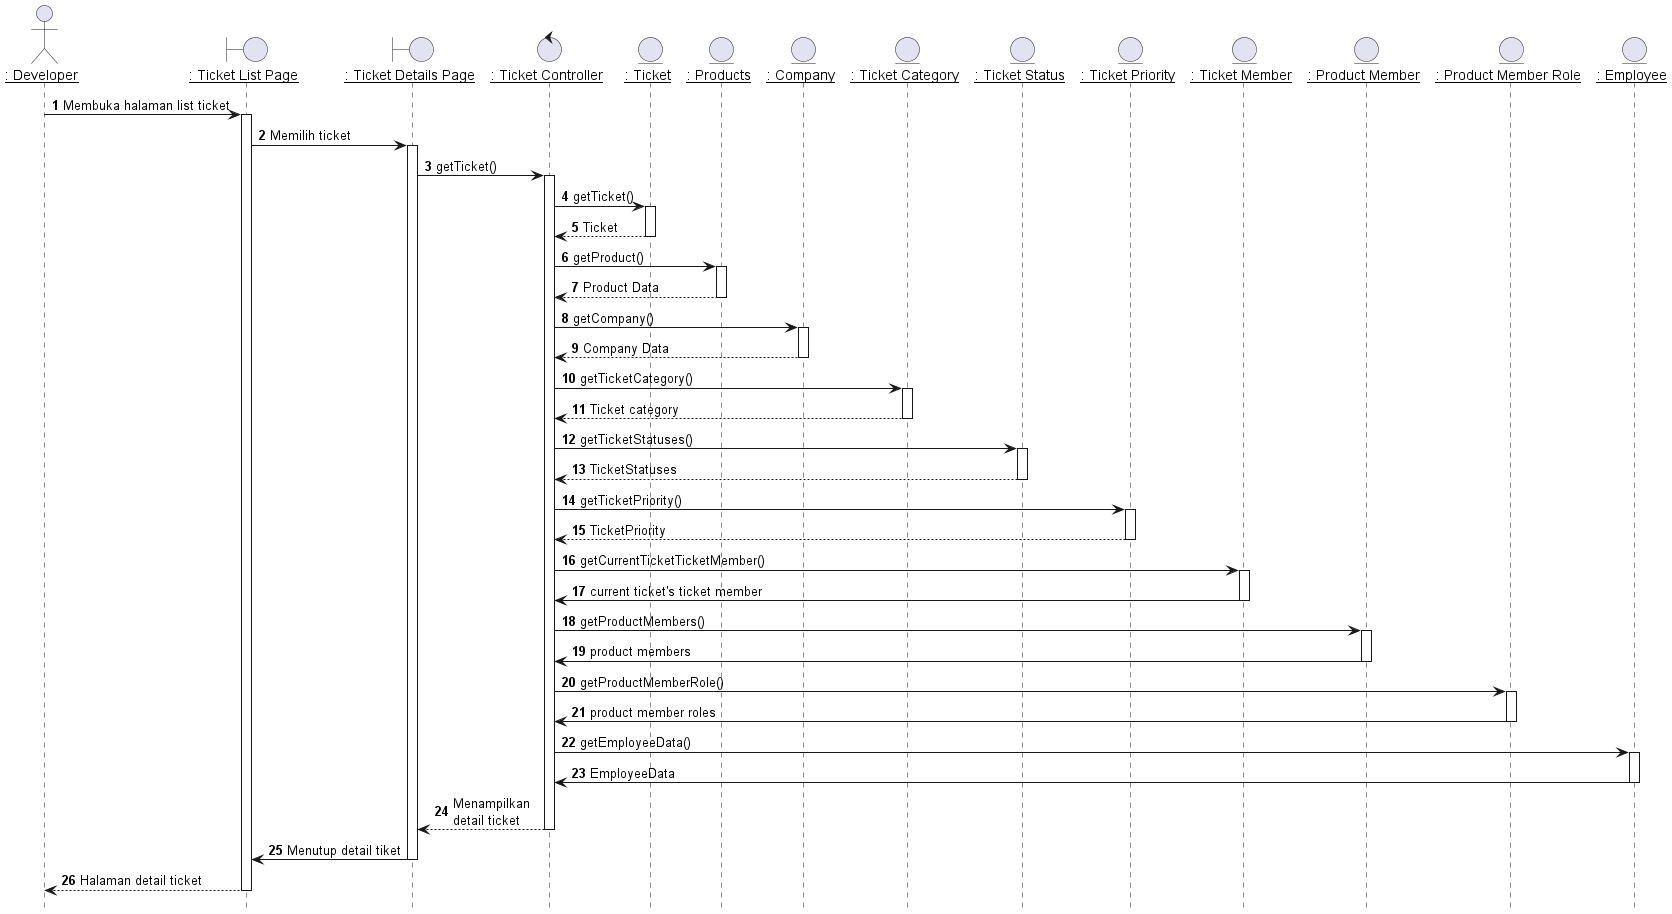
\includegraphics[width=\textwidth]{out/plantuml/sequence/idev/idev3/Melihat Detail Ticket.png}
                    \caption{Sequence Diagram Melihat Detail Ticket (DEV)}
                    \label{fig:SQ-DEV-03}
                \end{sidewaysfigure}

                \begin{sidewaysfigure}
                    \centering 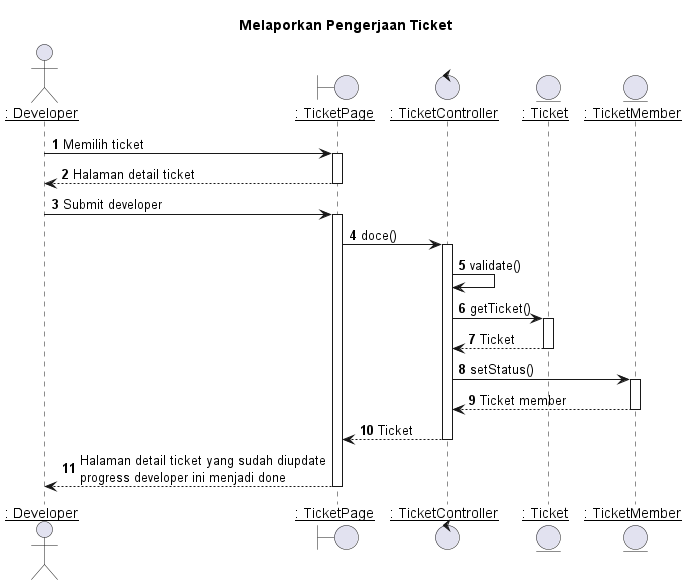
\includegraphics[width=\textwidth]{out/plantuml/sequence/idev/idev4/Melaporkan Pengerjaan Ticket.png}
                    \caption{Sequence Diagram Melaportkan Pengerjaan Ticket (DEV)}
                    \label{fig:SQ-DEV-04}
                \end{sidewaysfigure}
            \end{enumerate}

            \listsection{Sequence Diagram External User}
            \begin{enumerate}[label=\arabic*., wide]
                \item Sequence Diagram Melihat List Ticket
                
                \begin{sidewaysfigure}
                    \centering 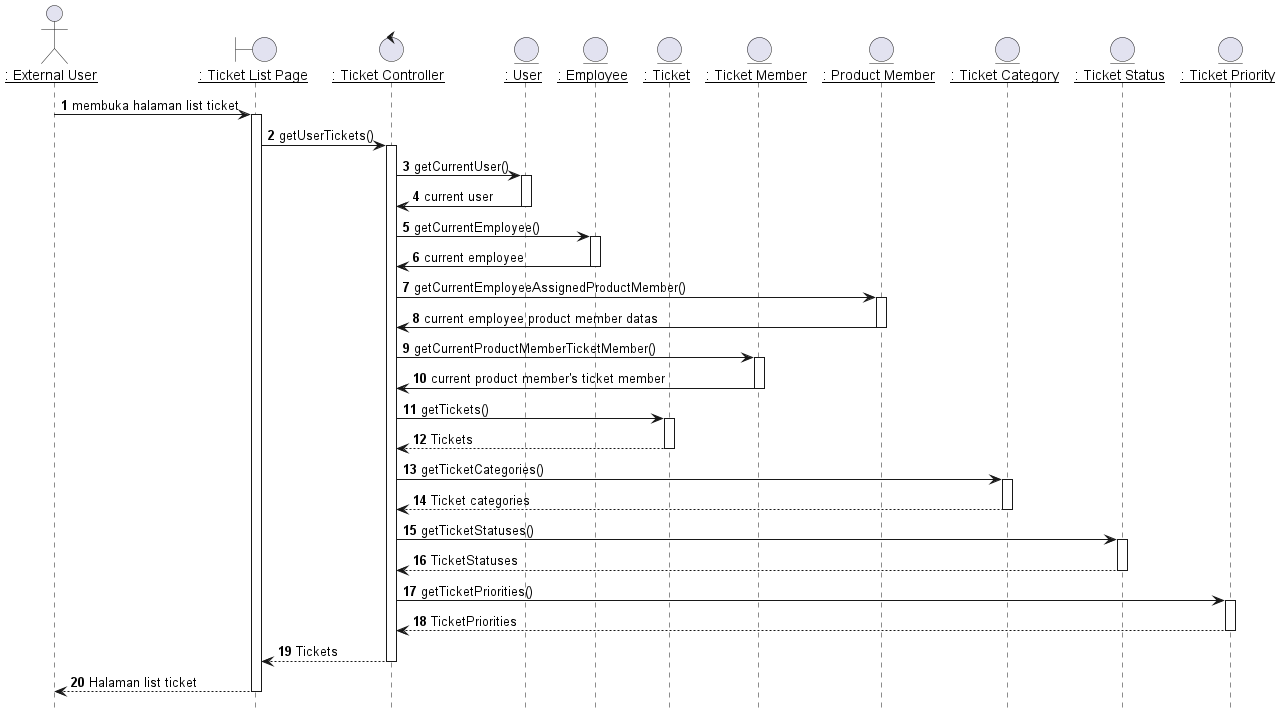
\includegraphics[width=\textwidth]{out/plantuml/sequence/ex/ex1/Melihat List Ticket.png}
                    \caption{Sequence Diagram Melihat List Ticket (External User)}
                    \label{fig:SQ-PIC-01}
                \end{sidewaysfigure}

                \begin{sidewaysfigure}
                    \centering 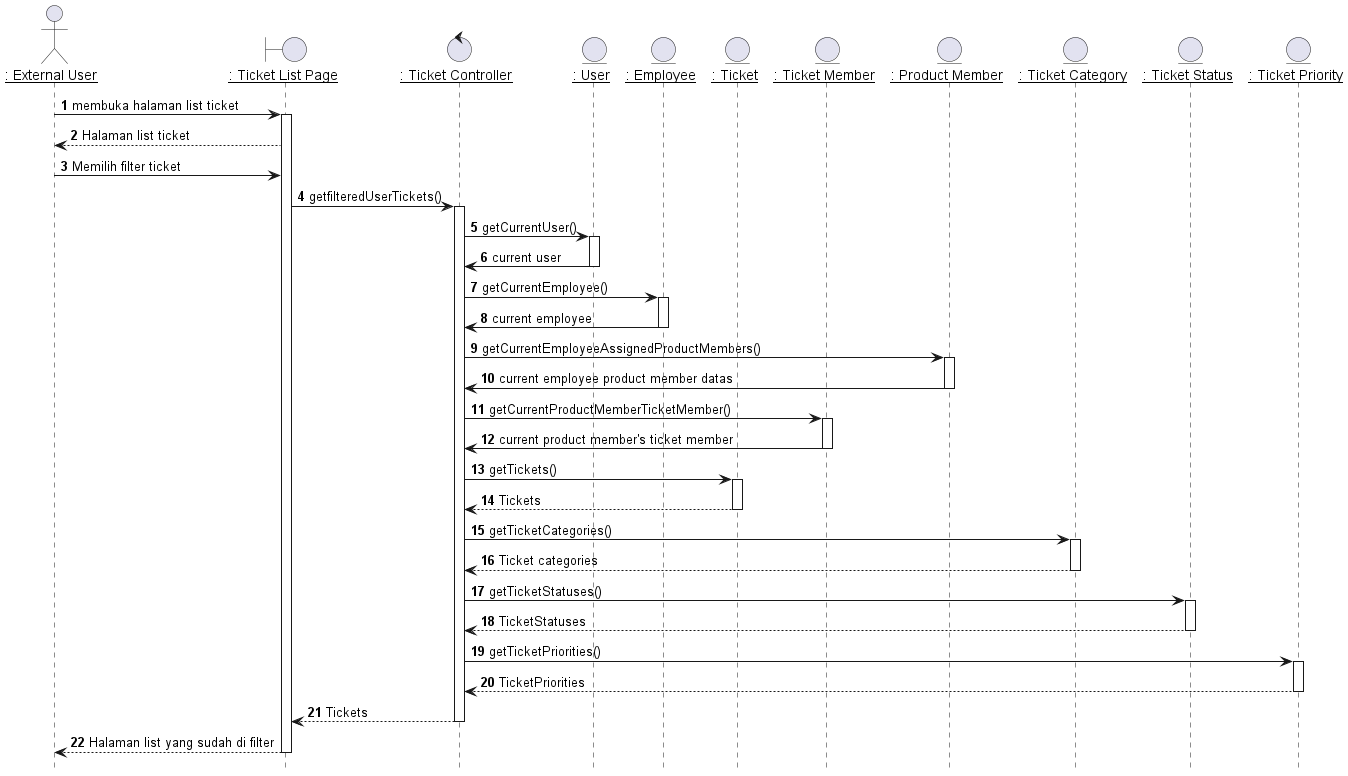
\includegraphics[width=\textwidth]{out/plantuml/sequence/ex/ex2/Memfilter List Ticket.png}
                    \caption{Sequence Diagram Memfilter List Ticket (External User)}
                    \label{fig:SQ-PIC-02}
                \end{sidewaysfigure}

                \begin{sidewaysfigure}
                    \centering 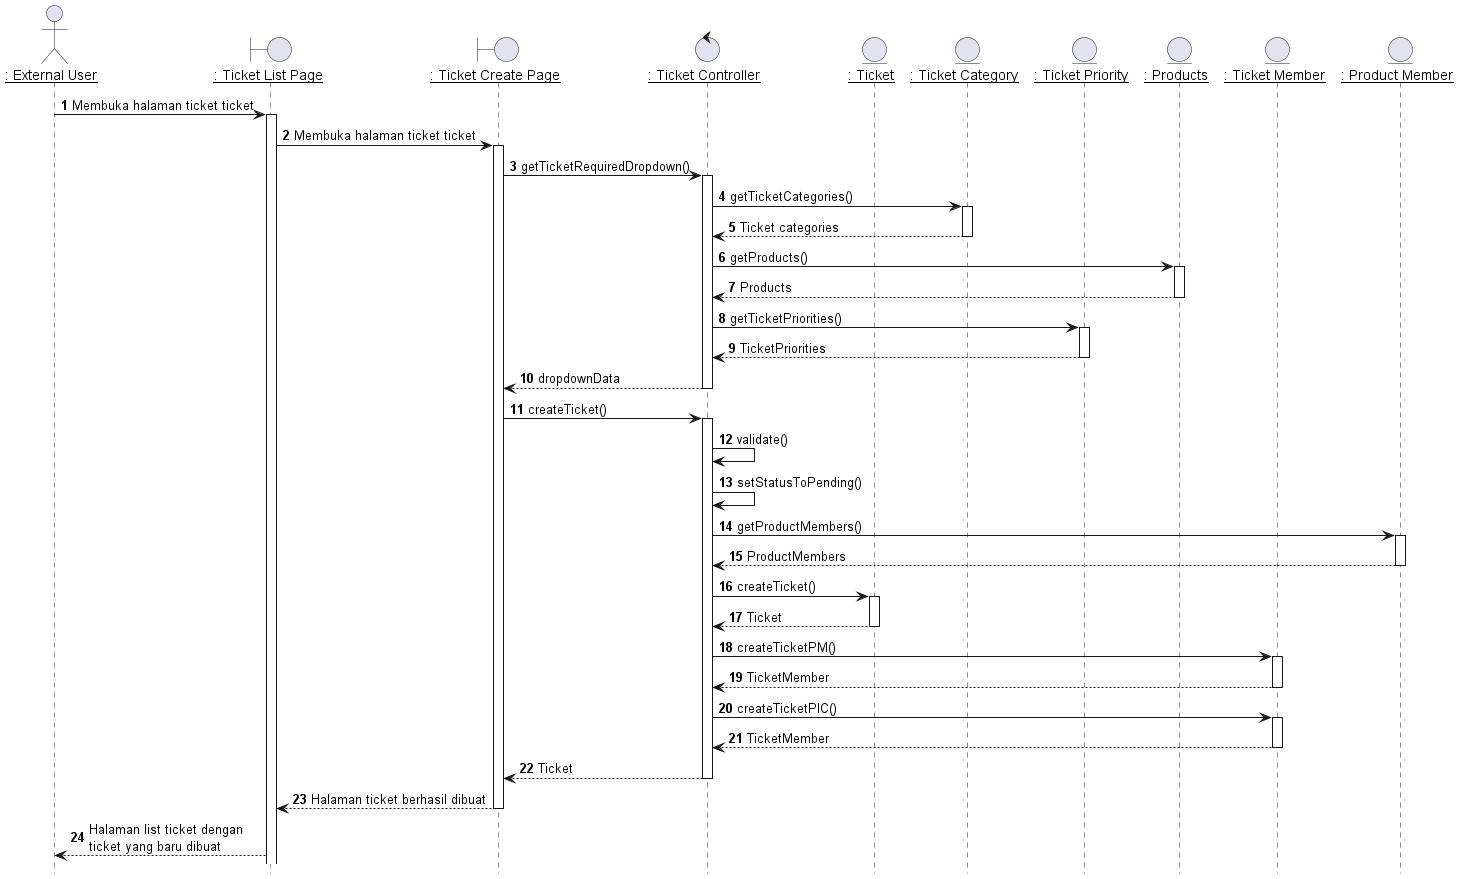
\includegraphics[width=\textwidth]{out/plantuml/sequence/ex/ex3/Membuat Ticket.png}
                    \caption{Sequence Diagram Membuat Ticket (External User)}
                    \label{fig:SQ-PIC-03}
                \end{sidewaysfigure}

                \begin{sidewaysfigure}
                    \centering 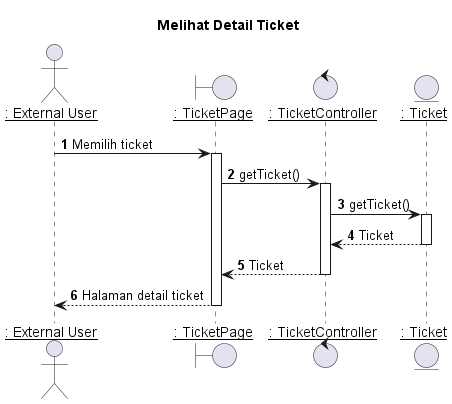
\includegraphics[width=\textwidth]{out/plantuml/sequence/ex/ex4/Melihat Detail Ticket.png}
                    \caption{Sequence Diagram Melihat Detail Ticket (External User)}
                    \label{fig:SQ-PIC-04}
                \end{sidewaysfigure}

                \begin{sidewaysfigure}
                    \centering 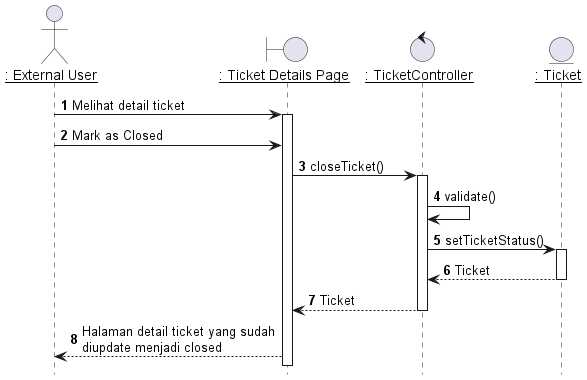
\includegraphics[width=\textwidth]{out/plantuml/sequence/ex/ex5/Menutup Ticket.png}
                    \caption{Sequence Diagram Menutup Ticket (External User)}
                    \label{fig:SQ-PIC-05}
                \end{sidewaysfigure}

                \begin{sidewaysfigure}
                    \centering 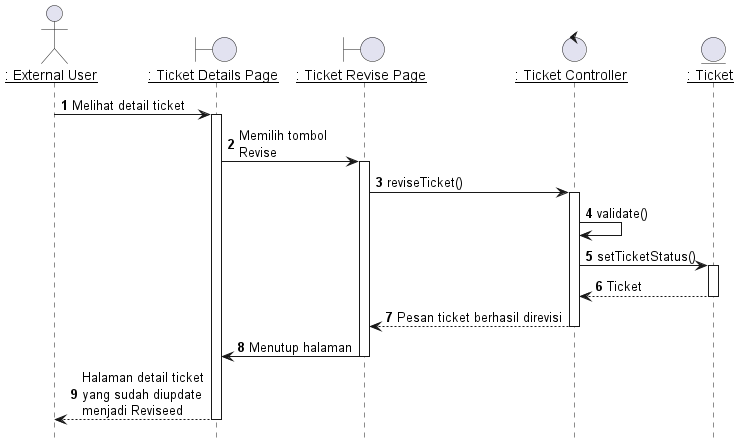
\includegraphics[width=\textwidth]{out/plantuml/sequence/ex/ex6/Merevisi Ticket.png}
                    \caption{Sequence Diagram Merevisi Ticket (External User)}
                    \label{fig:SQ-PIC-06}
                \end{sidewaysfigure}

                \begin{sidewaysfigure}
                    \centering 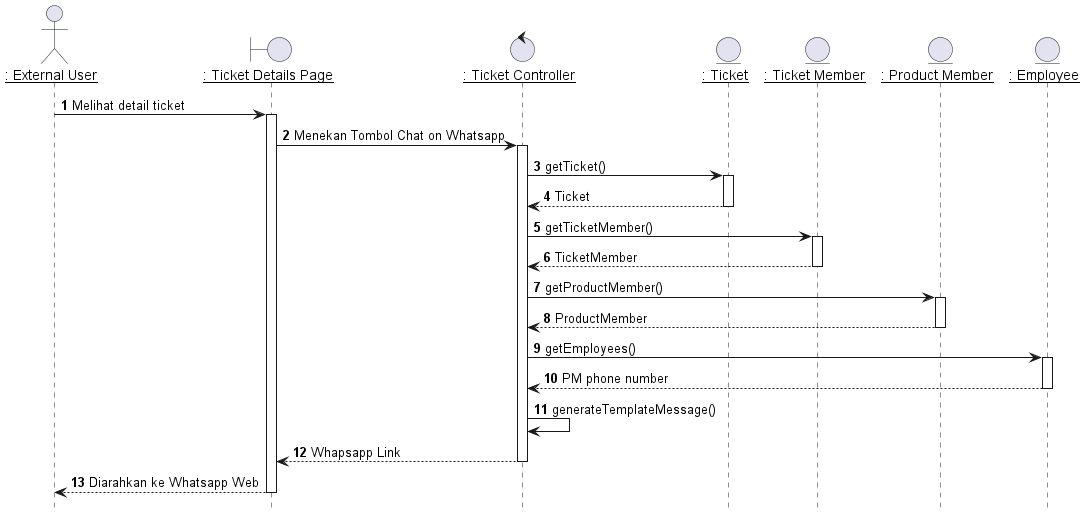
\includegraphics[width=\textwidth]{out/plantuml/sequence/ex/ex7/Berkomunikasi Dengan PM Melalui Whatsapp.png}
                    \caption{Sequence Diagram Berkomunikasi Dengan PM Melalui Whatsapp (External User)}
                    \label{fig:SQ-PIC-07}
                \end{sidewaysfigure}
            \end{enumerate}

        \end{enumerate}

          
    \end{enumerate}

    asd \citep{doe2021} dan  \citep{smith2020}

    
    \newpage

\end{enumerate}


\newpage


\section{BAB V\\HASIL DAN PEMBAHASAN}

% \begin{center}
% {
%     \setstretch{2}
%     \textbf{\large BAB IV} \\
%     \textbf{\large PENUTUP} \\
% }
% \end{center}

\begin{enumerate}[label=\textbf{4.\arabic*}]
    \item \textbf{Kesimpulan} \\
    Dalam praktikum ini, kami mempelajari konsep dasar Style dan Theme di android yang membantu untuk 
    mengurangi duplikasi kode yang berada di file Layout. Kami juga mempelajari constrained layout
    yang bisa mempermudah penataan agar posisi dari setiap widget dapat flexible dan mengikuti 
    aturan yang sudah di berikan

\end{enumerate}

\newpage

\bibliographystyle{plainnat}
\bibliography{references}


\end{document}
